\documentclass[conference]{IEEEtran}
\bibliographystyle{IEEEtran}
\linespread{1.2}
\usepackage[margin = 1.25 in]{geometry}
\usepackage{wrapfig}
\usepackage{amsfonts}
\usepackage[utf8]{inputenc}
\usepackage[T1]{fontenc}
\usepackage{graphicx}
\usepackage[english]{babel}
\usepackage[algoruled]{algorithm2e}

\renewcommand{\theequation}{\thesection.arabic{equation}}

\renewcommand{\thefigure}{\thesection.\arabic{figure}}



\renewcommand{\vec}[1]{\mathbf{#1}}
\renewcommand{\theequation}{\thesubsection.\arabic{equation}}
\DeclareGraphicsExtensions{.pdf,.png,.jpg, .gif}

\usepackage{amsthm}

\usepackage[english]{babel}
\usepackage{mathtools}

%\usepackage[OT2,T1]{fontenc}
%\DeclareSymbolFont{cyrletters}{OT2}{wncyr}{m}{n}
%\DeclareMathSymbol{\sha}{\mathalpha}{cyrletters}{"58}

\DeclareFontFamily{U}{wncy}{}
\DeclareFontShape{U}{wncy}{m}{n}{<->wncyr10}{}
\DeclareSymbolFont{mcy}{U}{wncy}{m}{n}
\DeclareMathSymbol{\Sh}{\mathord}{mcy}{"58} 
\DeclareMathOperator*{\argmin}{arg\,min}

\newcounter{eqn}
\renewcommand*{\theeqn}{\alph{eqn})}
\newcommand{\num}{\refstepcounter{eqn}\text{\theeqn}\;}

\makeatother
\newcommand{\vectornorm}[1]{\left|\left|#1\right|\right|}
\newcommand*\conjugate[1]{\bar{#1}}

\newtheorem{thm}{Theorem}
\newtheorem{defn}{Definition}
 %\theoremstyle{plain}
  \newtheorem{theorem}{Theorem}[section]
  \newtheorem{corollary}[theorem]{Corollary}
  \newtheorem{proposition}[theorem]{Proposition}
  \newtheorem{lemma}[theorem]{Lemma}
\newtheorem{example}[theorem]{Example}
  \newtheorem{definition}[theorem]{Definition}
  \newtheorem{conj}[theorem]{Conjecture}
 \newtheorem{condition}{Condition}
 \newtheorem{remark}[theorem]{Remark}

\newcommand{\supp}{\operatorname{supp}} 
\newcommand{\vc}[1]{{\mathbf{ #1}}}
\newcommand{\tn}{\widetilde{\nabla}_{n} }
\newcommand{\Z}{{\mathbb{Z}}}
\newcommand{\re}{{\mathbb{R}}}
\newcommand{\II}{{\mathbb{I}}}
\newcommand{\ep}{{\mathbb{E}}}
\newcommand{\pr}{{\mathbb{P}}}
\newcommand{\FF}{{\mathcal{F}}}
\newcommand{\TT}{{\mathcal{T}}}
\newcommand{\phin}{\phig{n}}
\newcommand{\phig}[1]{\phi^{(#1)}}
\newcommand{\ol}[1]{\overline{#1}}
\newcommand{\eff}{{\rm eff}}
\newcommand{\suc}{{\rm suc}}
\newcommand{\tends}{\rightarrow \infty}
\newcommand{\setS}{{\mathcal{S}}}
\newcommand{\setP}{{\mathcal{P}}}
\newcommand{\setX}{{\mathcal{X}}}
\newcommand{\nec}{{\rm nec}}
\newcommand{\bd}{{\rm bd}}

\title{Distributed Wideband Spectrum Sensing}

\author{Thomas Kealy$^{1}$, Oliver Johnson$^{2}$ and Robert Piechocki$^{3}$% <-this % stops a space
\thanks{This work was supported by the Engineering and Physical Sciences Research Council [grant number {\tt EP/I028153/1}]; Ofcom; and the University of Bristol. The authors would particularly like to thank Gary Clemo of Ofcom for useful discussions.}%
\thanks{ $^{1}$Thomas Kealy is with CDT in Communications, MVB, School of Engineeering University of Bristol, UK
        {\tt\small tk12098@bristol.ac.uk}}%
\thanks{$^{2}$Oliver Johnson is with the Department of Mathematics, University Walk, Bristol, University of Bristol, UK.
        {\tt\small O.Johnson@bristol.ac.uk}}%
\thanks{$^{3}$Robert Piechocki is with the CSN Group, MVB, School of Engineering, University of Bristol, UK.
        {\tt\small r.j.piechocki@bristol.ac.uk}}%
}

\IEEEoverridecommandlockouts

\begin{document}

\maketitle

\begin{abstract}
\noindent We consider the problem of reconstructing wideband frequency spectra from distributed, compressive measurements. The measurements are made by a network of nodes, each independently mixing the ambient spectra with low frequency, random signals. The reconstruction takes place via local transmissions between nodes, each solving simple statistical 
\end{abstract}

\section{Introduction}
There is an almost ubiquitous need to send more data over wireless networks, with 4G now being rolled out in the UK and US and with 5G being planned for 2020 and beyond \cite{Dahlman2014}. There is constrained frequency set over which to transmit this information. This issue could be alleviated by users dynamically allocating spectrum on a per-transmission basis. However, we (in the UK) currently lack any mechanism by which we are able to gain knowledge of spectral conditions. Frequencies have historically been allocated via auction, organised by OFCOM, so devices are unable to make dynamic decisions about how to transmit this data. This leads to both spectral exhaustion on some frequencies whilst much of the available radio spectrum lies fallow.  

Dynamic spectrum access won't become a reality unless spectral holes can be robustly detected. OFCOM requires that secondary users exploit the new spectrum politely, without interference to primary user makes spectrum sensing essential to TV white-space (TVWS) technologies. The realisation of any Cognitive Radio standard (such as IEEE 802.22 \cite{stevenson2009ieee}), requires the co-existence of primary (TV users) and secondary (everybody else who wants to use TVWS spectrum) users of the frequency spectrum to ensure proper interference mitigation and appropriate network behaviour. 

Users of TVWS (Cognitive Radios) must sense whether spectrum is available, and must be able to detect very weak primary user signals. Furthermore they must sense over a wide bandwidth (due to the amount of TVWS spectrum proposed), which challenges traditional Nyquist sampling techniques, because the sampling rates required are not technically feasible with current RF or Analogue-to-Digital conversion technology.

Due to the inherent sparsity of spectral utilisation, Compressive Sensing (CS) \cite{Candes2006} is an appropriate formalism within which to tackle this problem. CS has recently emerged as a new sampling paradigm allowing images to be taken from a single pixel camera for example. Applying this to wireless communication, we are able to reconstruct sparse signals at sampling rates below what would be required by Nyquist theory. 

However, even with CS, spectrum sensing from a single machine will be costly as the proposed TVWS band will be over a GHz frequency range. CS at a single sensor would still require GHz sampling rates. In this paper we propose a distributed model, which allows a sensing budget at each node far below what is required by centralised CS. The main contribution of this paper is that the model can be solved in a fully distributed manner - we do not require a central fusion centre as in \cite{Zhang2011b}.

The structure of the paper is as follows: in section (\ref{sec:sensingmodel}) we introduce the sensing model, in section (\ref{sec:admm}) we describe the distributed reconstruction algorithm \cite{mota2013d}, and finally in section (\ref{sec:results}) we show some results of the reconstruction quality of this model. \cite{mishali2010theory} \cite{tropp2010beyond}

\section{Models}\label{sec:sensingmodel}

We consider a radio environment with a single primary user (PU) and a network of \(J\) nodes collaboratively trying to sense and reconstruct the PU signal, either in a fully distributed manner (by local communication), or by transmitting measurements to a fusion centre which then solves the linear system. 

We try to sense and reconstruct a wideband signal, divided into \(L\) channels. We have a (connected) network of \(J\) (= 50) nodes placed uniformly at random within the square \(  \left[0,1\right]\times \left[0,1\right] \). This is the same model as in \cite{Zhang2011b}.

The nodes individually take measurements (as in \cite{mishali2010theory}) by mixing the incoming analogue signal \(x\left(t\right)\) with a mixing function \(p_i\left(t\right)\) aliasing the spectrum. \(x\left(t\right)\) is assumed to be bandlimited and composed of up to \(k\) uncorrelated transmissions over the \(L\) possible narrowband channels - i.e. the signal is \(k\)-sparse. 

The mixing functions - which are independent for each node - are required to be periodic, with period \(T_p\). Since \(p_i\) is periodic it has Fourier expansion:

\begin{equation}
p_i\left(t\right) = \sum_{l=-\infty}^{\infty} c_{il} \exp\left({jlt\frac{2\pi}{T_p}}\right)
\end{equation}

The \(c_{il}\) are the Fourier coefficients of the expansion and are defined in the standard manner. The result of the mixing procedure in channel \(i\) is therefore the product \(xp_i\), with Fourier transform:

\begin{align}
X_{i}\left(f\right) &=& \int_{-\infty}^{\infty} x\left(t\right) p_i\left(t\right) dt
\\ &=& \sum_{l=-\infty}^{\infty} c_{il} X\left(f-lf_p\right)
\end{align}

(We insert the Fourier series for \(p_i\), then exchange the sum and integral). The output of this mixing process then, is a linear combination of shifted copies of \(X\left(f\right)\), with at most \(\lceil f_NYQ/f_p\rceil\) terms since \(X\left(f\right)\) is zero outside its support (we have assumed this Nyquist frequency exists, even though we never sample at that rate).

This process is repeated in parallel at each node so that each band in \(x\) appears in baseband.

Once the mixing process has been completed the signal in each channel is low-pass filtered and sampled at a rate \(f_s \geq f_p\). In the frequency domain this is a ideal rectangle function, so the output of a single channel is:

\begin{equation}
Y_i\left(e^{j 2 \pi f T_s }\right) = \sum_{l = -L_0}^{+L_0} c_{il} X\left(f-lf_p\right)
\end{equation}

since frequencies outside of \([-f_s/2, f_s/2]\) will filtered out. \(L_0\) is the smallest integer number of non-zero contributions in \(X\left(f\right)\) over \([-f_s/2, f_s/2]\) - at most \(\lceil f_NYQ/f_p\rceil\) if we choose \(f_s = f_p\). These relations can be written in matrix form as:

\begin{equation}
\textbf{y} = \textbf{A}\textbf{x} + \vec{w}
\label{system}
\end{equation}

where \(\textbf{y}\) contains the output of the measurement process, and \(\textbf{A}\) is a product matrix of the mixing functions, their Fourier coefficients, a partial Fourier Matrix, and a matrix of channel coefficients. \(\textbf{x}\) is the vector of unknown samples of \(x\left(t\right)\). 

i.e. \(\textbf{A}\) can be written: 

\begin{equation}
\textbf{A}^{m\times L} = \textbf{S}^{m\times L} \textbf{F}^{L\times L} \textbf{D}^{L \times L} \textbf{H}^{L \times L}
\end{equation}

The measurements \(\textbf{y}\) are transmitted to a Fusion Centre via a control channel. The system  \ref{system} can then be solved (in the sense of finding the sparse vector \(\vec{x}\) by convex optimisation via minimising the objective function:

\begin{equation}
\frac{1}{2}\|\textbf{Ax}-\textbf{y}\|_2^2 + \lambda \|\textbf{x}\|_1
\end{equation}

where \(\lambda\) is a parameter chosen to promote sparsity. 

\section{ADMM }\label{sec:admm}
The alternating direction method of multipliers \cite{Boyd2010a}, (ADMM), algorithm solves problems of the form

\begin{align}
\text{min}_{x} f\left( x \right) + g\left(z\right)
\\
\text{s.t } Ux +Vz = c
\label{admm}
\end{align}

where \(f\) and \(g\) are assumed to be convex function with range in \(\re\), \(U \in \re^{p \times n}\) and \(V\in \re^{p \times m}\) are matrices (not assumed to have full rank), and \(c \in \re^p\).

ADMM consists of iteratively minimising the augmented Lagrangian 

\begin{align*}
L_p\left(x, z, \eta\right) = f\left( x\right) +& g\left(z\right)+\eta^T\left(Ux+Vz-c\right) + \\ \frac{\rho}{2}\|Ux+Vz-c\|_2^2
\label{admm_form}
\end{align*}

(\(\eta\) is a Lagrange multiplier) with the following iterations:

\begin{align}
x^{k+1} &:= \argmin_{x} L_\rho\left(x,z^k,y^k\right)\\
z^{k+1} &:= \argmin_{z} L_\rho\left(x^{k+1},z,y^k\right)\\
\eta^{k+1} &:= \eta^{k} + \rho \left(Ux^{k+1} + Vz^{k+1} - c\right)
\label{admm_algo}
\end{align}

The alternating minimisation works because of the decomposability of the objective function: the \(x\) minimisation step is independent of the \(z\) minimisation step and vice versa.  

We illustrate an example, relevant to the type of problems encountered in signal processing.

\subsection{Example: ADMM for Centralised LASSO}
ADMM can be formulated as an iterative MAP estimation procedure for the problem (which is referred to as LASSO see \cite{tibshirani1996regression}):

\begin{eqnarray}
\frac{1}{2}\|Ax-b\|_2^2 + \lambda\|x\|_1
\end{eqnarray}

This can be cast in constrained form as:

\begin{eqnarray}
\frac{1}{2}\|Ax-b\|_2^2 + \lambda\|z\|_1 \\
\text{s.t } z = x
\end{eqnarray}

i.e this is of the form \eqref{admm_form} with \( f\left(x\right) =\|Ax-y\|_2^2\), \(g\left(z\right) = \lambda\|z\|_1\), \(A=B=I\), and \(c=0\).

and the associated Lagrangian is:

\begin{equation}
L_\rho = \frac{1}{2}\|Ax-b\|_2^2 + \lambda\|z\|_1 + \eta\left(x-z\right) + \frac{\rho}{2}\|x-z\|^2
\label{eq:lasso-lagrangian}
\end{equation}

Now, given a set of noisy measurements (say of radio spectra) \(\vec{y}\), and a sensing matrix \(\vec{A}\) we can use ADMM to find the (sparse) radio spectra.

The ADMM iterations for LASSO, which can be found by alternately differentiating \eqref{eq:lasso-lagrangian} with respect to \(x\),\(z\) and \(\lambda\), are (in closed form):

\begin{align}
x^{k+1} &:= \left(A^TA + \rho I\right)^{-1}\left(A^Tb +\rho\left(z^k - y^k\right)\right)\\
z^{k+1} &:= S_{\lambda/\rho}\left(x^{k+1} + y^k/\rho\right)
 \\
y^{k+1} &:= y^{k} + \rho \left(x^{k+1}-z^{k+1}\right)
\label{admm_algo_lasso}
\end{align}

where \(S_{\lambda/\rho}\left(\circ\right)\) is the soft thresholding operator: \(S_\gamma\left(x\right)_i = sign(x_i)\left(|x_i| - \gamma\right)^+\).

This algorithm has a nice statistical interpretation: it iteratively performs ridge regression, followed by shrinkage towards zero. Exactly like the MAP estimate for LASSO problem under a Laplace prior.

The soft-thresholding operator can be derived by considering the MAP estimate of the following model:

\begin{equation}
y = x + w
\end{equation}

where \(x\) is some (sparse) signal, and \(w\) is additive white Gaussian noise. We seek

\begin{equation}
\hat{x} = \arg\max_x \pr_{x|y}{\left(x|y\right)}
\end{equation}

This can be recast in the following form by using Bayes rule, noting that the denominator is independent of \(x\) and taking logarithms:

\begin{equation}
\hat{x} = \arg\max_x \left[\log{\pr_{n}{\left(y-x\right)}}+\log{\pr{\left(x\right)}}\right]
\label{hatx}
\end{equation}

The term \(\pr_{n}{\left(y-x\right)}\) arises because we are considering \(x+w\) with \(w\) zero mean Gaussian, with variance \(\sigma_n^2\). So, the conditional distribution of \(y\) (given \(x\)) will be a Gaussian centred at \(x\).

We will take \(\pr{\left(x\right)}\) to be a Laplacian distribution:

\begin{equation}
\pr{\left(x\right)} = \frac{1}{\sqrt{2}\sigma}\exp{-\frac{\sqrt{2}}{\sigma}|x|}
\end{equation}

Note that \( f\left(x\right) = \log{\pr_x{ \left( x \right)}} ~ -\frac{\sqrt{2}}{\sigma} |x| \), and so by differentiating \( f'\left(x\right) = -\frac{\sqrt{2}}{\sigma} sign\left(x\right) \)

Taking the maximum of \ref{hatx} we obtain:

\begin{equation}
\frac{y-\hat{x}}{\sigma^2_n}-\frac{\sqrt{2}}{\sigma}sign(x) = 0
\end{equation}

Which leads the soft thresholding operation defined earlier, with \(\gamma = \frac{\sqrt{2}\sigma^2_n}{\sigma}\) as (via rearrangement):

$$
y =  \hat{x} + \frac{\sqrt{2}\sigma^2_n}{\sigma}sign\left(x\right)
$$

or

$$
\hat{x}\left(y\right) = sign(y)\left(y - \frac{\sqrt{2}\sigma^2_n}{\sigma}\right)_+
$$

\section{Constrained Optimisation on Graphs}
We model the network as an undirected graph \(G = \left(V,E\right)\), where \(V = \{1 \ldots J\}\) is the set of vertices, and \(E = V \times V\) is the set of edges. An edge between nodes \(i\) and \(j\) implies that the two nodes can communicate. The set of nodes node \(i\) can communicate with is written \(\mathcal{N}_i\) and the degree of node \(i\) is \(D_i = |\mathcal{N}_i|\). 

We assume that a proper (or approximate) colouring of the graph is available: that is each node is assigned a number from a set \(C = \{1 \ldots c \} \), and no node shares a colour with any neighbour.

Given the measurement model from the section (\ref{sec:sensingmodel}), we can represent the linear system by concatenating the measurements of each node into a single system. Here each row of the matrix represents the measurements of a single node. I.e we are trying to solve the following problem:

\begin{equation}
\text{min} f\left(x\right) \text{ subject to } A_p x = y_p
\end{equation}

where \(f\) is some global function we seek to minimise, \(A_p\) is the row of the sensing matrix \(A\) available to node \(p\), and \(y_p\) are the measurements taken by node \(p\).

The problem is coupled at each node by the variable \(x\). To ease this issue, at each node create a local copy, denoted \(x_j\) (so there will be \(J\) copies of this variable). Then, for consistency, we constrain the problem so that each copy is identical: \(x_1 = x_2 = \ldots x_J\). Equivalently, given the graphical structure of the problem, we require that \(x_i = x_j\) for each edge of the network.

So now we are solving the problem


\begin{align}
\text{min}_{x} \frac{1}{J}\sum_J f_p\left(x_j\right)
\\
\text{s.t } A_p x_p = y_p \text{ and } x_i = x_j \text{ if } \{i,j\} \in E 
\label{ constrainedbp}
\end{align}

where \(f_p\) is a copy of the global function \(f\) stored at node \(p\).

This is exactly the kind of problem that can be attacked by the Alternating Direction Method of Multipliers, described previously. We present a short example for bipartite graphs, which can easily be generalised to graphs with many colours. 
 
\subsection{Example: bipartite graphs}
We are here considering graphs which are connected, and 2-colourable, that is nodes 1 to \(c\) have colour 1 (red say), and nodes \(c+1\) to \(J\) have colour 2 (blue). We will demonstrate that we can decompose problem (\ref{constrainedbp}) into \(c\) problems which can be executed in parallel by minimising \(x\) at the 1st set of nodes, and \(J - c\) problems which also can be executed in parallel by minimising at the second set of nodes. 

Firstly, for compactness, we introduced the arc-incidence matrix of the graph \(B\). This is the \(J \times E\) matrix where each column corresponds to an edge \(\{i,j\} \in E\), with the \(ith\) and \(jth\) entries equal to 1 and -1 respectively. With this notation, we can rewrite (\ref{constrainedbp}) as:

\begin{equation}
\text{min} \frac{1}{J}\sum_J f_p\left(x_j\right) \text{ subject to } A_p x_p = y_p \text{ and } \left(B^T \circ I \right)\bar{x} = 0 
 \label{constrainedbp1}
\end{equation}

where \(\bar{x} = \left(x_1, x_2, \ldots x_c \right)\), and \(\circ\) is the Kronecker product. 

In this form, the updates for each node (within a colour) of the problem (\ref{constrainedbp1}) can be written in the following way:

\begin{align*}
\bar{x}_p^{k+1} = \frac{1}{J}\sum_{j \in C_i} f_p\left(x_j\right) + \phi_1\left(\bar{x}_i, \lambda\right)
\end{align*}
where 

\begin{align*}
\phi_i\left(\bar{x}_i, \lambda\right) &= \lambda^T\left(B_i^T\circ I_n\right)\bar{x}_i + \frac{\rho}{2}\vectornorm{\left(B_i^T\circ I_n\right)\bar{x}_i }^2 \\
&= \left(\left(B_i^T\circ I_n\right)\lambda \right)^T\bar{x}_i + \frac{\rho}{2}\bar{x}_i^T\left(B_1B_2^T\circ I_n\right)\bar{x}_i
\end{align*}

Since, no nodes within \(C_i\) are neighbours \(B_iB_i^T\) is a diagonal matrix (with the degree of node \(i\) as the \(i\)th entry). So, we can finally re-write

\begin{equation*}
\phi_i\left(\bar{x}_i, \lambda\right) = \sum_{j \in C_i}\left(\left(\sum_{k \in \mathcal{N}_i} sign\left(k-i\right)\lambda_{\{i,k\}}\right)^T x_i + \frac{\rho}{2}D_i\vectornorm{x_i}^2  \right)
\end{equation*}

where the dual variable \(\lambda\) has been decomposed edge-wise so that \(\lambda_{\{i,j\}} = \lambda_{\{j,i\}}\) and is associated with edge \(\{i,j\}\) and the constraint \(x_i = x_j\). This function \(\sum_{p \in C_c} f_p\left(x_p\right) + \phi_i\left(\bar{x}_i, \lambda\right)\) is what is minimised at each node within each colour (in parallel). For LASSO take \(f_p := \|Ax_p-b_p\|_2^2 + \frac{\beta}{J}\|x_p\|_1 \).


\section{Results} \label{sec:results}

The model described in section (\ref{sec:sensingmodel}) was simulated, with a wideband signal of 201 channels and a network of 50 nodes (i.e. the signal will be sampled at a 1/4 of rate predicted by Nyquist theory). The mixing patterns were generated from iid Gaussian sources (i.e the matrix S had each entry drawn from an iid Gaussian source). Monte Carlo simulations were performed at EbN0db values ranging from 5 to -5 in steps of 1, and the expected Mean Squared Error (MSE) of solutions of a centralised solver (spgl1) and a distributed solver (ADMM). The results can be seen in fig (\ref{msevssnr1}). 

These results indicate that for both centralised and distributed solvers, adding noise to the system results in a degrading of performance. Interestingly note, that the distributed solver seems to (slightly) outperform the centralised solver at all SNRs. This is counter-intuitive, as it would be expected that centralised solvers knowing \textit{all} the available information would outperform distributed solutions. We conjecture that the updates described in section \ref{optongraphs}, take into account differences in noise across the network. The distributed averaging steps, which form the new prior for each node, then penalise updates from relatively more noisy observations. This corroborates observations from \cite{bazerque2008}.

This observation is (partially) confirmed in figure (\ref{erroriterations}), which plots the progress of the centralised and distributed solvers (as a function of iterations) towards the optimum solution. The SNR is 0.5 (i.e the signal is twice as strong as the noise).

\begin{figure}[h]
\centering
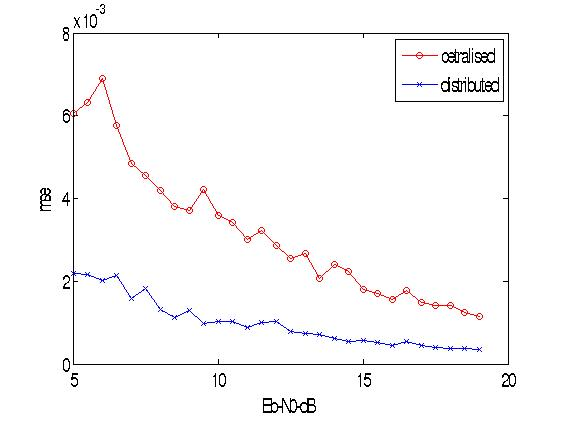
\includegraphics[height = 5 cm]{centvsdistmsegaussian10perpoint.jpg}
\caption{Mse vs SNR for the 'frequency only sensing model, showing the performance of distributed and centralised solvers}
\label{msevssnr1}
\end{figure}

\begin{figure}[h]
\centering
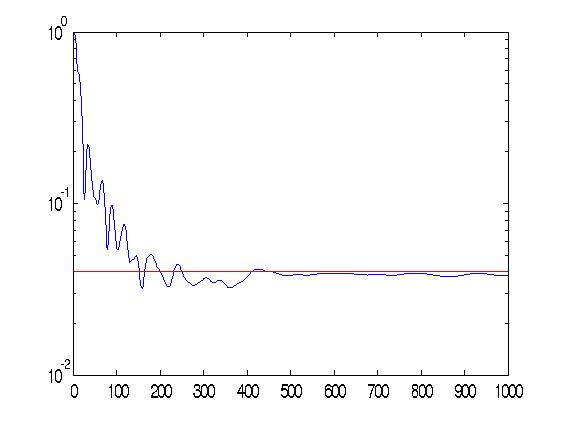
\includegraphics[height = 5 cm]{erroriterations1.jpg}
\caption{The progress of a distributed and a centralised solver as a function of the number of iterations }
\label{erroriterations}
\end{figure}

\bibliography{cswireless1}

\end{document}